\section{Parallelization, Distribution, and Grouping}
\label{sec:parallelization}

\subsection{Parallelization}
 To handle large scale, processing has to be done in parallel and distributed among many machines. Thus, Stream processing systems break applications and streams into smaller units. An application is composed of many independent operators, and each operator has several parallel instances (Figure \ref{fig:stream}). Similarly, a stream is composed of several \textit{partitions}. Figure \ref{fig:parallelization}-a shows an example dataflow with partitions $\{P_{AB}\_1, P_{AB}\_2, P_{AB}\_3\}$. \Fix{how about when they all have similar duplicate input?}
Each instance autonomously operators on a separate partition of the input stream (e.g., $B_1$ on $P_{AB}\_1$), and produces output to partitions of an output stream (e.g., $A_1$ outputting to all partitions ). 

\subsection{Distribution}
Stream applications are distributed across a cluster of processing \textit{nodes}, as shown in Figure \ref{fig:parallelization}-b. Typically, each instance is treated as a single thread \footnote{Some systems use a different variation of instance to thread mapping. For example, Storm enables mapping multiple instances to a thread, and Samza used to provide a single thread (per process) model \Fix{cite}.}. 
Instances are placed together into a \textit{process} or container (which is essentially a process), and then processes are distributed across nodes. Note that in a given node, process of a given application or two different applications may run concurrently. 
Section \Fix{X and Y} discuss the different placement and distribution strategies used for both instances and processes. 
\Fix{should this be here? or move to another section}
	
\begin{figure}[t]
	\centering
	\subfigure[Parallelization and partitioning]{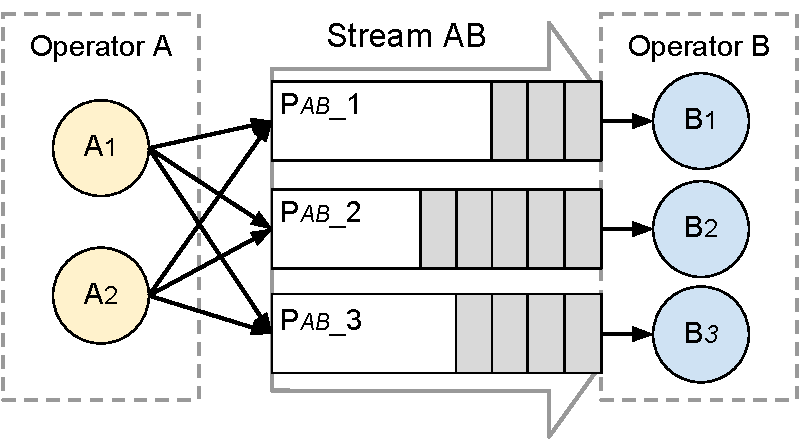
\includegraphics[width=0.45\linewidth]{partition}}
	\hspace*{1cm}
	\subfigure[Distribution]{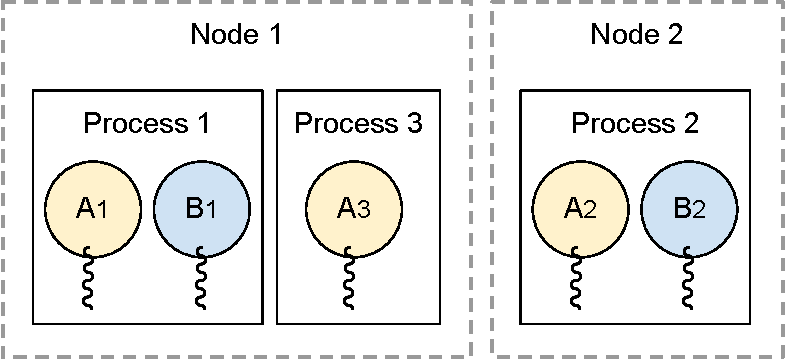
\includegraphics[width=0.45\linewidth]{distibution} 
	}
	\caption{An example application with two operators, A and B, with: a) the parallelization of operators into instances (A = $\{A_1, A_2\}$, B =$\{B_1, B_2, B_3\}$) and partitioning of the AB Stream, and b) the distribution of instances among processing nodes.}
\label{fig:parallelization}
	
\end{figure}

\subsection{Grouping}

\noindent \textbf{Definition:} As shown in Figure \ref{fig:parallelization}-a, an operator instance ($A_1$) outputs items to all partitions of an output stream. The \textit{grouping} strategy defines which partition(s) an output item should be added to. Grouping are defined per stream. An operator with various input streams might have different grouping in each.

\noindent \textbf{\\Solutions, trade-offs and usecases:}
For a given instance $o_s$ of $O_{src}$ generating item $i$ to $O_{dst}$, through output stream $s$ with partitions $P_s=\{p_1, p_2, ..., p_k\}$, the common groupings are:
\begin{itemize}
	\item \textbf{Random:} where $i$ is randomly assigned to one of the partitions in $P_s$. Random grouping guarantees load balance among partitions in terms of number of items. However, this approach is unaware of the placement of instances (locality unaware). This grouping is one of the most common groupings.
	\item \textbf{Hash-based:} where using a consistent hashing on the item's key, $i$ is hashed to one of the partitions in $P_s$. \Fix{define item's key}. This grouping guarantees all items with the same key go to the same partition (thus, processed by one instance). This is a commonly used grouping and necessary feature when doing joins or aggregations over a specific key. However, poor hashing and skewed data can create load imbalance.
	
	\Fix{@ le: there is another mode of hash-based (Partial Key grouping: ) along with load balancing. I think it belongs to the load balancing section or should be removed entirely. it is based on this paper:
	https://melmeric.files.wordpress.com/2014/11/the-power-of-both-choices-practical-load-balancing-for-distributed-stream-processing-engines.pdf	
	}

	\item \textbf{All:} where $i$ is replicated and sent to \textit{all} partitions. This grouping acts as a broadcast, and should be used with care because of its high overhead. This is mostly useful for sending coordination and management messages.
	\item \textbf{One:} where all items, such as $i$,  are sent to one specific partition, e.g, $p_1$. This is mostly used when all data needs to be aggregated at one processor. However, it create huge load-imbalance. This is a special case of Hash-based grouping.
	\item \textbf{Locality aware:} where placement of instances are considered in sending $i$. If an instance $o_d$ of $O_{dst}$ is placed on the same process as where $o_s$ is placed, $i$ is sent to $o_d$. Otherwise, a random instance of $O_{dst}$ is chosen. This approach minimizes network traffic and latency. However poor placements can create load imbalance.


	

	Local or shuffle grouping: If the target bolt has one or more tasks in the same worker process, tuples will be shuffled to just those in-process tasks. Otherwise, this acts like a normal shuffle grouping.
\end{itemize}

Stream processing frameworks mostly support all these groupings. Table \ref{table:grouping} summarizes the groupings, their trade-offs, and the systems providing them.

\begin{table}[h]
	\tbl{Grouping solutions and their trade-offs	\label{table:grouping}}{
		\tiny		
		\begin{tabular}{p{.1 \linewidth}|p{.2 \linewidth}|p{.45 \linewidth}|p{0.07 \linewidth}}%
			
			\hline
			\rowcolor[HTML]{E0E0E0} 
			Solution	&Description&Trade-offs & Usecase
			\csvreader[head to column names]{tables/grouping.csv}{}% use head of csv as column names
			{\\\hline\textbf{\csvcoli} & \csvcolii & \csvcoliii & \csvcoliv}% specify your coloumns here
			\\ \hline
		\end{tabular}	
	}
\end{table}



\noindent \textbf{\\Future Direction:}  
\Fix{is there any?}